% -*- mode: latex -*-
\mansection{xsetech}
\begin{mandesc}
  \short{xsetech}{set parameters of a subwindow in a graphic window}\\ 
\end{mandesc}
%-- Calling sequence section
\begin{calling_sequence}
\begin{verbatim}
  xsetech(wrect,[frect,logflag])  
  xsetech(options=value)
\end{verbatim}
\end{calling_sequence}
%-- Parameters
\begin{parameters}
  \begin{varlist}
    \vname{a3d}: a boolean. If \verb!%t! it means that the subwindow is used for 3D plots.
    \vname{arect}: vector of size 4.
    \vname{axesflag}: an integer 
    \vname{clip}: a boolean 
    \vname{fixed}: a boolean 
    \vname{frect}: vector of size 4.
    \vname{frect}: vector of size 4.  
    \vname{iso}: a boolean 
    \vname{logflag}: string of length 2 \verb!"xy"!, where x and y can be \verb!n! or 
    \verb!l!. Character \verb!n! stands for normal and \verb!l! stands for logscale. x stands
    for the x-axis and y stands for the y-axis.
    \vname{arect}: vector of size 4.
    \vname{wrect}: vector of size 4.
  \end{varlist}
\end{parameters}

\begin{mandescription}
  The function \verb!xsetech! is used to set parameters of a graphic subwindow 
  which will be used for plotting. 
  \begin{description} 
    \item[a3d]: If true this boolean indicated that the subwindow is used for 3D plots.
    \item[arect] the parameter \verb!arect=[axleft, axright,ayup,aydown]!
      is used to describe the graphic frame inside the subwindow. The graphic frame is specified (like
      \verb!wrect!) using proportion of the width or height of the current
      graphic subwindow (default value is \verb!1/8*[1,1,1,1]!). 
    \item[axesflag]: a integer parameter which fix the way scales are displayed.
    \item[clip]: If true this boolean indicated that graphics are to be clipped inside the graphic frame 
      (described by \verb!arect!).
    \item[fixed]: If true this boolean indicated that the scales specified by \verb!frect! are fixed i.e 
      they won't be changed by subsequent calls to plot functions. 
    \item[frect] the parameter \verb!frect=[xmin,ymin,xmax,ymax]! gives the scale to be used for drawing 
      (default value of is \verb![0,0,1,1]!).
    \item[iso]: If true this boolean indicated that the scales should provide iso mode 
    \item[logflag]: log scale specification.
    \item[wrect] the parameter \verb!wrect=[xleft,yup,w,h]! is used to describe the subwindow poisition 
      in the graphic windows (See figure below).  The fours values in the vector \verb!wrect! are 
      numbers in the range $(0,1)$ which gives dimensions as proportion of the width or height of the graphic window. 
      For instance \verb!wrect=[0,0,1,1]! means that the whole graphics window will be used by the graphic subwindow
      and \verb!wrect=[0.5,0,0.5,1]! means that the graphic subwindow will be the half right of the graphics window.
      Default value of is \verb![0,0,1,1]!.
    \end{description}

    \begin{center}
    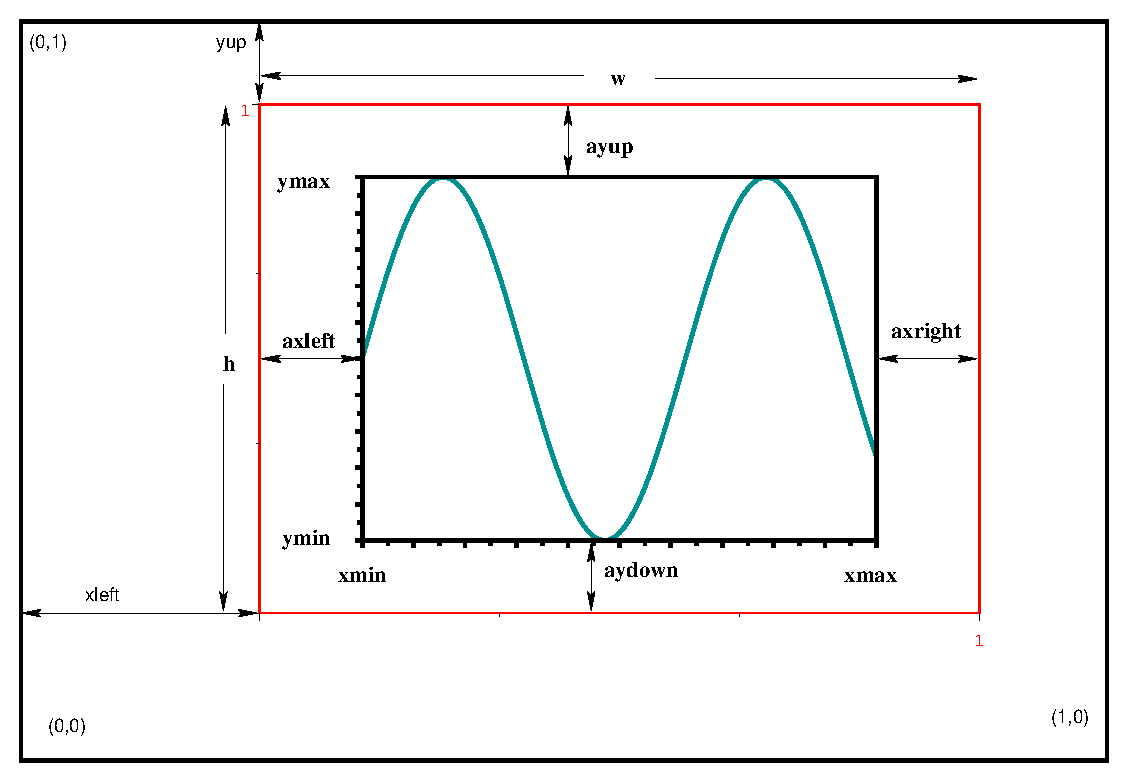
\includegraphics{\mansrc graphics/xsetechfig}
    \end{center}
\end{mandescription}

%--example
\begin{examples}

\noindent two subwindows 

\begin{mintednsp}{nsp}
  xsetech(wrect=[0,0,1.0,0.5],frect=[-5,-3,5,3])
  plot2d([1:10]',[1:10]',style=1,strf="001")
  xsetech(wrect=[0,0.5,1.0,0.5],axesflag=4)
  plot2d([1:10]',[1:10]',strf='014',rect=[-6,-6,6,6]);
\end{mintednsp}

\noindent four subwindows

\begin{mintednsp}{nsp}
  xsetech(wrect=[0,0,0.5,0.5],a3d=%t); plot3d()
  xsetech(wrect=[0.5,0,0.5,0.5]); plot2d()
  xsetech(wrect=[0.5,0.5,0.5,0.5]); grayplot()
  xsetech(wrect=[0,0.5,0.5,0.5]); histplot()
\end{mintednsp}

\noindent using \verb!arect!

\begin{mintednsp}{nsp}
  xsetech(wrect=[0,0,1.0,0.5],arect=1/8*ones(1,4));
  x=1:0.1:10;plot2d(x',sin(x)');
  xsetech(wrect=[0,0.5,1.0,0.5],arect=[2/8,2/8,1/16,1/4]);
  x=1:0.1:10;plot2d(x',sin(x)');
\end{mintednsp}
\end{examples}
%-- see also
\begin{manseealso}
  \manlink{xgetech}{xgetech} \manlink{subplot}{subplot} \manlink{isoview}{isoview} \manlink{square}{square} 
\end{manseealso}
%-- Author

\begin{authors}
  J.-Ph. C.  
\end{authors}

